%قبل از شروع مسئله ترجیحاً چیزی ننویسید. اما اگر خواستید بنویسید، در قالب لیستی (فقرات و شمارش) بنویسید.
%برای اضافه کردن نمره، بعدی از شروع‌مسئله، [x] را اضافه کنید و به جای x نمره مورد نظر را قرار دهید. برای زیرمسئله‌ها هم به همین صورت است.


%\شروع‌مسئله[10]
\شروع‌مسئله [14]
\\
شنگدباو همانطور که در سؤالات قبلی مشخص بود علاقه خاصی به جمع کردن گوی دارد! دیوار اتاق شنگدباو دیواری
$n \times W$
است که ارتفاعش $n$ است و عرض آن برابر $W$ است. شنگدباو برای راحتی کارش هر نقطه از این دیوار را با یک سیستم مختصات نشان می‌دهد. بالای دیوار اتاقش روی سقف تعدادی سوراخ وجود دارد این سوراخ‌ها به قطر ۱ در سقف قرار دارد. گاهی اوقات از یکی از این سوراخ‌ها گویی به پایین رها می‌شود و این گوی بین دو تا از خطوط عمودی مختصات سقوط می‌کند تا به زمین برسد.

اتاق شنگدباو تعدادی تاقچه دارد. در واقع در هر ارتفاعی یک تاقچه دارد که یا به سمت راست خم شده یا به سمت چپ. این تاقچه‌ها در شکل زیر نمایان‌اند به شکل یک خط هستند که دو سر آن مختصاتی صحیح دارد. اگر توپی هنگام سقوط به یکی از این تاقچه‌ها برخورد کند روی آن سر می‌خورد و یا از سمت راست یا از سمت چپ تاقچه به سقوط ادامه می‌دهد.

\begin{center}
	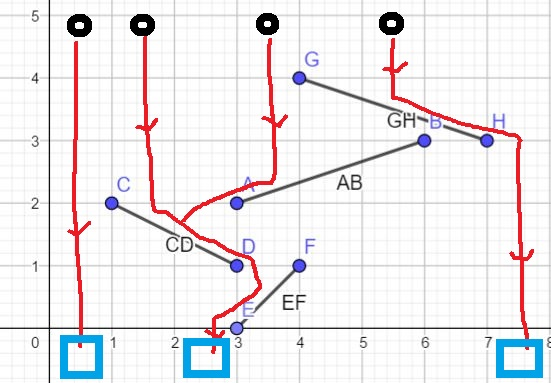
\includegraphics[scale=1]{src/toop}
	
	در شکل تعداد سوراخ‌های سقف ۴ تا و تعداد سبد‌ها ۳ تاست و این مقدار کمینه است.
\end{center}

شکل تاقچه‌ها و نقاط سوراخ روی سقف به شما داده‌شده است. (فرض کنید تعداد نقاط سوراخ روی سقف برابر $m$ تاست) 

شنگدباو می‌خواهد تعدادی سبد بر روی زمین بگذارد به طوریکه هر گوی در نهایت در یکی از این سبد‌ها بیفتد. کمترین تعداد سبد‌ها و جایگاه سبد‌ها را در حداکثر
$O((n + m) log (n + m))$
خروجی دهید.


%\متن‌سیاه{سوال عملی اول:}\\
%\متن‌سیاه{دراپ‌تست}\\

%\متن‌سیاه{ورودی:}\\
%در خط اول ورودی، ابتدا k و سپس m داده می‌شود.\\
%\متن‌سیاه{خروجی:}\\
%در تنها سطر خروجی، تعداد آیفون‌های مورد نیاز می‌آید. اگر در هیچ صورتی چنین کاری ممکن نبود ۱- چاپ می‌شود.\\
%\متن‌سیاه{محدودیت‌ها:}\\
%$1\leq k\leq 10^4$

%$m\leq10^9$
%\\
%\textbf{\متن‌سیاه{ورودی و خروجی نمونه}\\
%% تست اول
%\begin{latin}
% \begin{tabularx}{\textwidth}{|X | X|}
% \hline
% \textbf{stdin} &
% \textbf{stdout}\\
% \hline
% 100 100&
% 1\\
% \hline
% 
% \end{tabularx}
%\end{latin}
%
%% تست دوم
%
%\begin{latin}
% \begin{tabularx}{\textwidth}{|X | X|}
% \hline
% \textbf{stdin} &
% \textbf{stdout}\\
% \hline
% 340 20&
% 3\\
% \hline
% 
% \end{tabularx}
%\end{latin}}
% صورت اصلی مسئله را در این‌جا بنویسید.



\solution{
	فرض کنید نقاط روی سقف به ترتیب 
	$x_1, x_2, ..., x_m$
	هستند مجموعه $S$ را ابتدا برابر مختصات $x$ این نقاط قرار می‌دهیم. تاقچه‌ها را از بالا به پایین مرتب می‌کنیم و هر سری مجموعه $S$ را بروزرسانی می‌کنیم به طوریکه در لایه‌ای که هم اکنون هستیم توپ‌ها دقیقاً از مختصات داخل $S$ به پایین می‌لغزند روی آن‌ها پیمایش می‌کنیم هنگامی که به تاقچه $i$ ام می‌رسیم فرض کنید این تاقچه در بازه
	$[xl_i, xr_i]$
	است. در اینصورت همه اعضای $S$ که در این بازه هستند به این بازه برخورد کرده و یا به سمت چپ یعنی
	$xl_i$
	و یا به سمت راست یعنی
	$xr_i$
	می‌افتند بنابراین همه اعضا در این بازه را تبدیل به چنین چیزی می‌کنیم. در نهایت وقتی به زمین می‌رسیم $|S|$ جواب مسئله خواهد بود.
	
	فرض کنید اعضای $S$ را داخل یک درخت جست‌وجوی دودویی می‌ریزیم و هر سری کوچکترین عضو بزرگتر مساوی 
	$xl_i$
	را به‌دست می‌آوریم و روی اعضا به صورت مرتب‌شده (میان ترتیب) پیمایش می‌کنیم تا به آخرین عضو کمتر مساوی $xr_i$ برسیم. سپس همه این اعضا را حذف می‌کنیم و با توجه به جهت کج بودن تاقچه $xl_i$ یا $xr_i$ را به درخت اضافه می‌کنیم. 
	
	در مجموع حداکثر $n+m$ بار حذف یا اضافه کردن به درخت جست‌وجو داریم و پیدا کردن کوچکترین عضو بزرگتر مساوی
	$xl_i$
	یا رفتن به عدد بعدی در پیمایش میان‌ترتیب حداکثر لگاریتم اندازه درخت طول می‌کشد لذا الگوریتم از
	$\mathcal{O}((n + m) log (n + m))$
	است.
	
	
}

%%%%%%%%%%%%%%%%%%%%%%%%%%%%%%%%%%%%%%%%%%%%%%%%%%%%%
% برخی دستورات مفید برای تمرین‌ها. %
%%%%%%%%%%%%%%%%%%%%%%%%%%%%%%%%%%%%%%%%%%%%%%%%%%%%%

% فرمول‌های نمونه:
%$f(x) = \Theta(x)$
%$T(x, y) \leq \log(x) + 2^y + \binom{2n}{n}$
% {\tt code\_function}


% لیست موارد بدون شماره‌گذاری:
%\شروع{فقرات}
% \فقره مورد اول 
% \شروع{فقرات}
% \فقره مورد اول داخلی 
% \شروع{فقرات}
% \فقره اولین مورد خیلی داخلی 
% \فقره دومین مورد خیلی داخلی 
% \پایان{فقرات}
% \فقره مورد دوم داخلی 
% \پایان{فقرات}
% \فقره مورد دوم 
%\پایان{فقرات}

% لیست موارد شماره‌گذاری شده:
%\شروع{شمارش}
% \فقره یک مورد 
% \فقره یک مورد دیگر 
% \فقره باز هم یک مورد دیگر
%\پایان{شمارش}

% برای نوشتن یک فرمول چند خطی که یک شماره بخوره. برای حالت‌های دیگر به سایت زیر مراجعه کنید:
% https://www.overleaf.com/learn/latex/Aligning_equations_with_amsmath
%\begin{align} 
% \begin{split}
% (x+y)^3 &= (x+y)^2(x+y) \\
% &= (x^2+2xy+y^2)(x+y) \\
% &= (x^3+2x^2y+xy^2) + (x^2y+2xy^2+y^3) \\
% &= x^3+3x^2y+3xy^2+y^3
% \end{split} 
%\end{align}

% نوشتن ماتریس و آرایه دوبعدی
%\begin{align}
% A = 
% \begin{bmatrix}
% A_{11} & A_{21} \\
% A_{21} & A_{22}
% \end{bmatrix}
%\end{align}

% اضافه کردن تصویر با شرح. برای اضافه کردن تصویر بدون شرح، فقط دستور درج‌تصویر را استفاده کنید.

%\پایان{زیرمسائل}

%کد زیر را ببینید.
%%\lstinputlisting{source_filename.py}
%\begin{latin}
%\begin{lstlisting}
%# Import the modules
%import sys
%import random
%
%ans = True
%
%while ans:
%question = raw_input("Ask the magic 8 ball a question: (press enter to quit) ")
%
%answers = random.randint(1,8)
%
%if question == "":
%sys.exit()
%
%elif answers == 1:
%print "It is certain"
%
%elif answers == 2:
%print "Outlook good"
%
%elif answers == 3:
%print "You may rely on it"
%
%elif answers == 4:
%print "Ask again later"
%
%elif answers == 5:
%print "Concentrate and ask again"
%
%elif answers == 6:
%print "Reply hazy, try again"
%
%elif answers == 7:
%print "My reply is no"
%
%elif answers == 8:
%print "My sources say no"
%\end{lstlisting}
%\end{latin}